\section{Sequenzen}
    \subsection{Neue Zeiterfassung}
        Eine neue Zeiterfassung wird hinzugefügt.
        Dies kann entweder durch Übergabe von Start- und Endzeit oder durch das Starten und spätere Stoppen eines Timers geschehen.
        Falls der Stundenzettel für den entsprechenden Monat noch nicht existiert wird er erstellt.
        Nur Proletarier und Supervisor dürfen diese Aktion durchführen.
        Außerdem können nur Zeiterfassungen für Monate hinzugefügt werden, für die der Stundenzettel unlocked ist oder noch nicht existiert.\\

        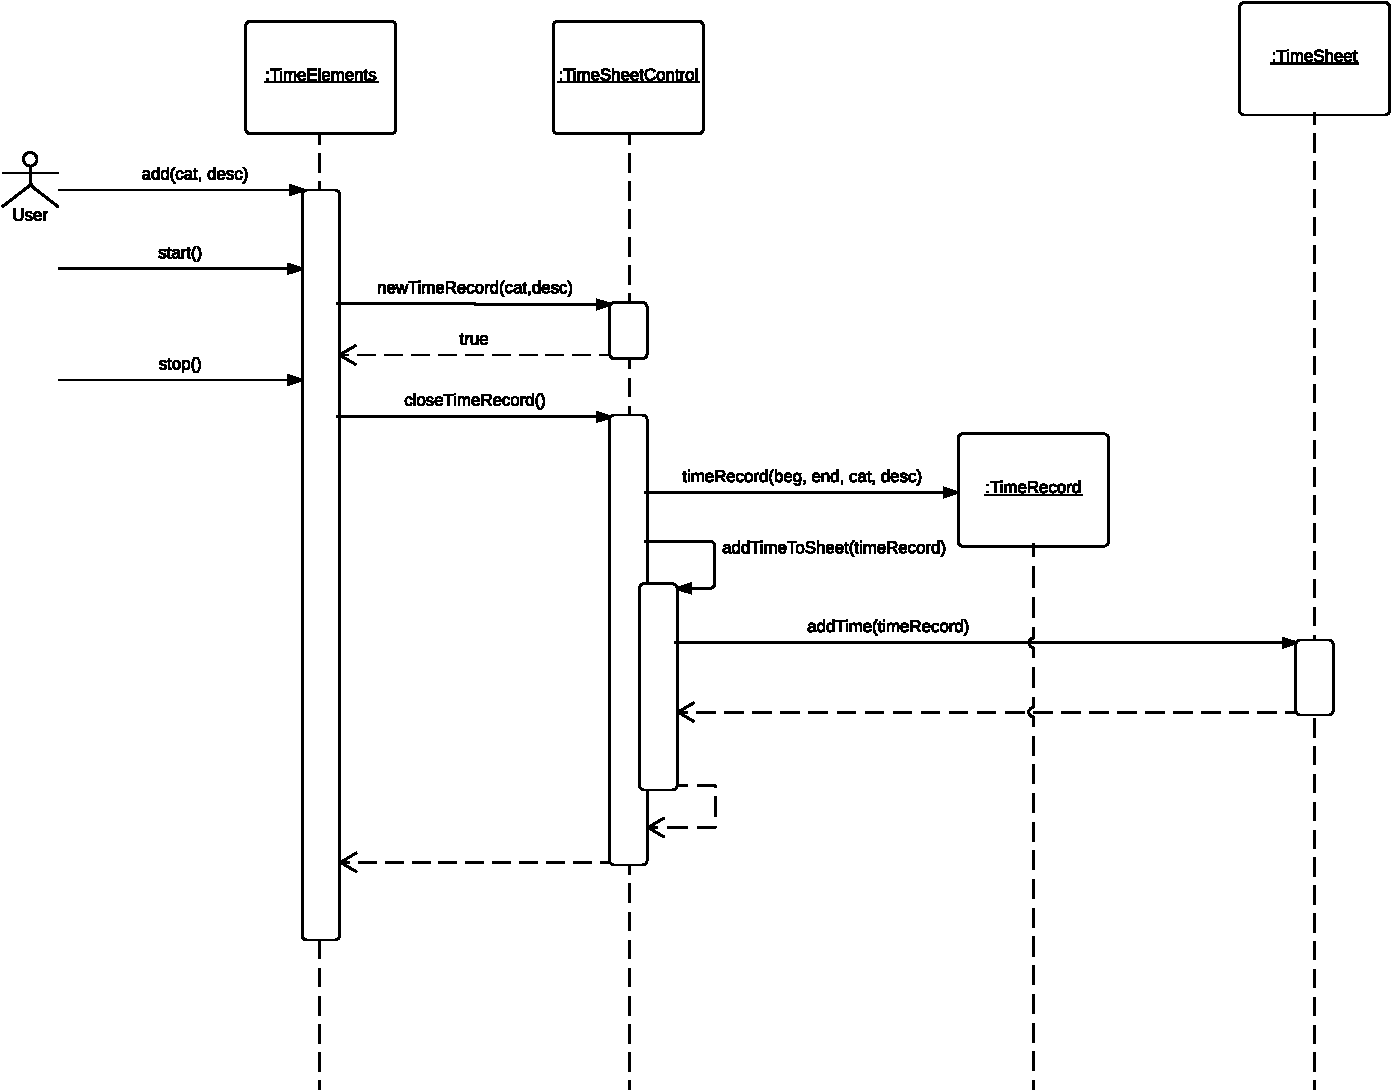
\includegraphics[width=\linewidth]{Diagramms/sequenzes/new_Time_record.pdf}

    \newpage
    \subsection{Login Sequenz}
        Ein User loggt sich ein.
        Falls als Authentifizierung LDAP statt Local ausgewählt ist, wird die Anfrage von LoginView stattdessen an den LDAP-Server weitergeleitet.
        Nur nicht eingeloggte User können diese Aktion durchführen.
        Für diese ist dies die einzige erlaubte Aktion.\\

        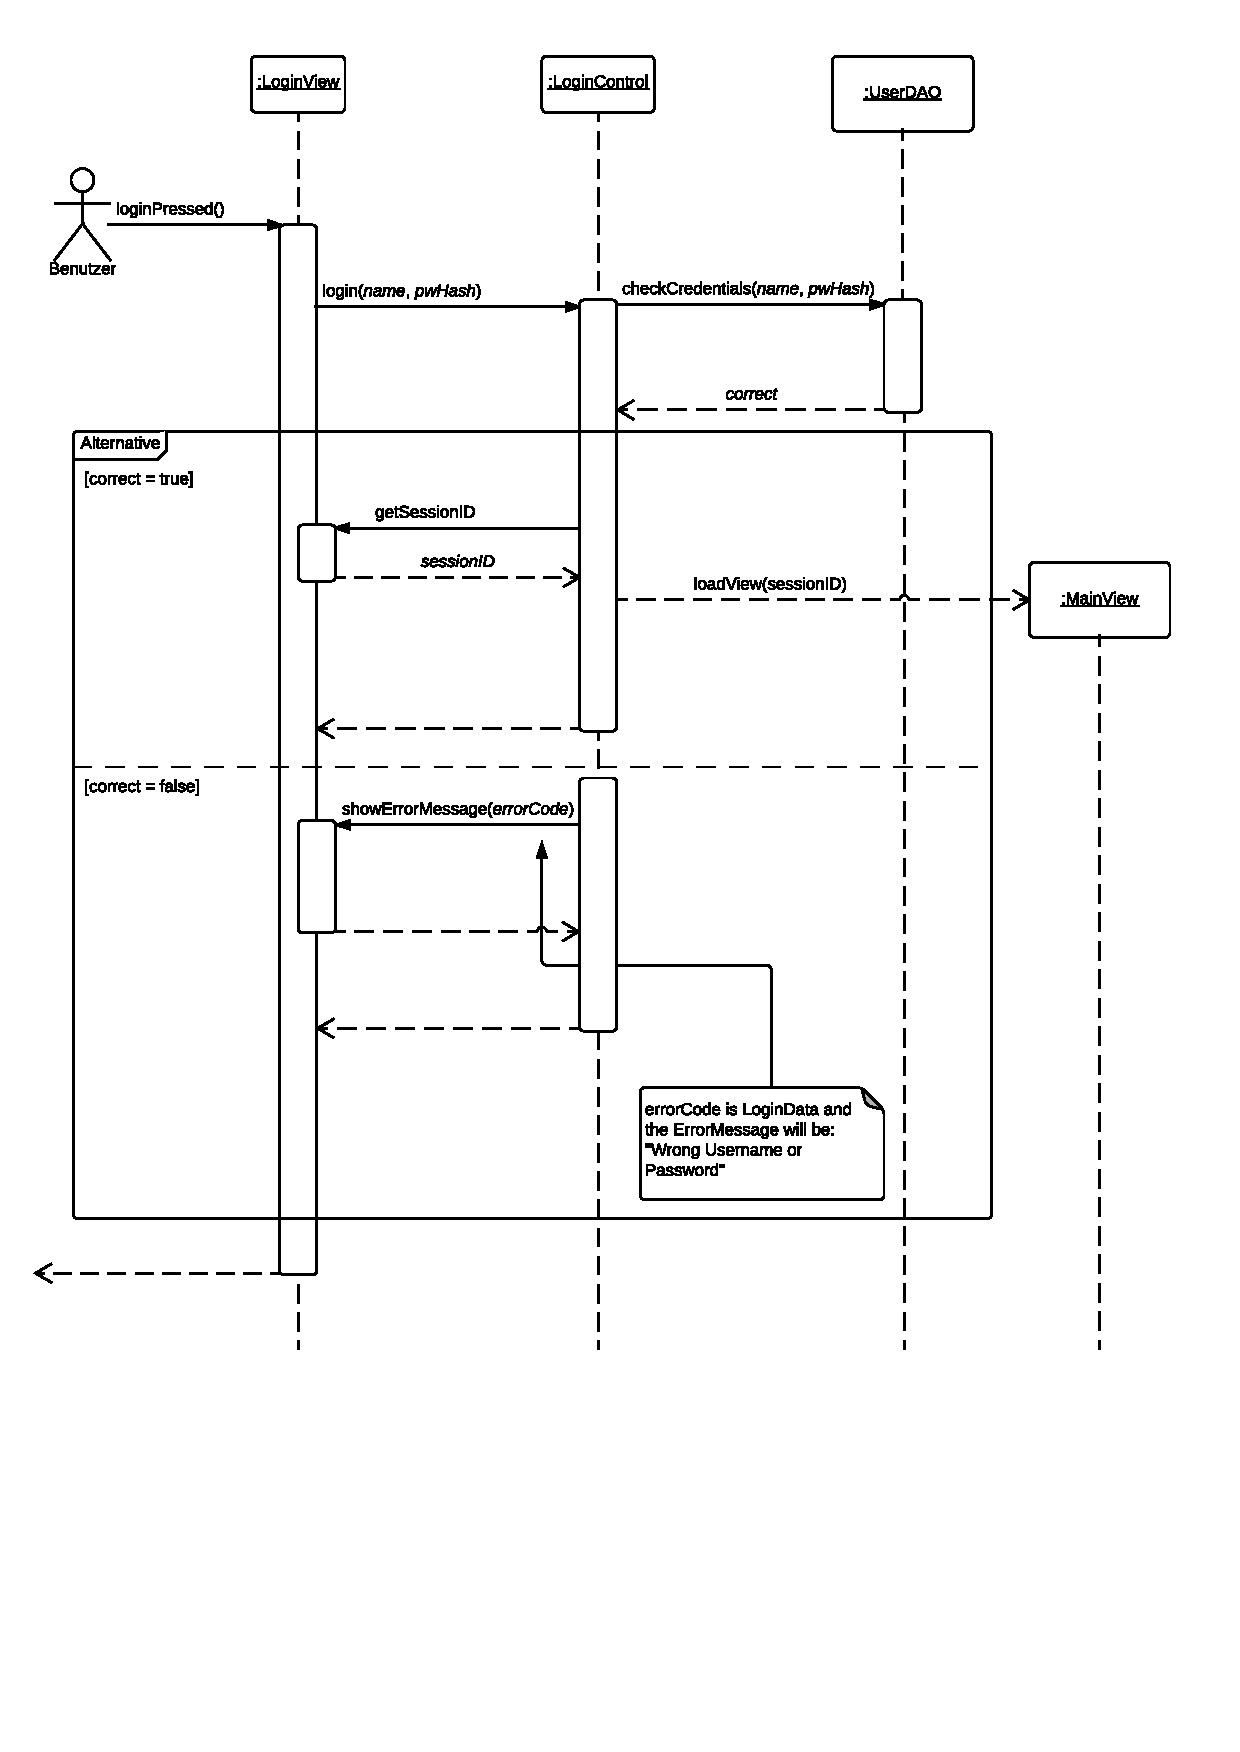
\includegraphics[width=\linewidth]{Diagramms/sequenzes/login.pdf}

    \newpage
    \subsection{Alle Stundenzettel der Gruppenmitglieder einsehen}
        Ein Supervisor lässt sich die Stundenzettel eines beliebigen Monats von allen von ihm betreuten Proletariern anzeigen.
        Supervisor können sich die Stundenzettel eines Monats von allen oder alle Stundenzettel eines von ihnen betreuten Proletariers anzeigen lassen.
        Administratoren können sich die Stundenzettel eines Monats aller Proletarier, nur aller von einem Supervisor betreuten Proletarier oder alle Stundenzettel eines Proletariers anzeigen lassen.
        Proletarier können diese Aktion nicht durchführen.\\

        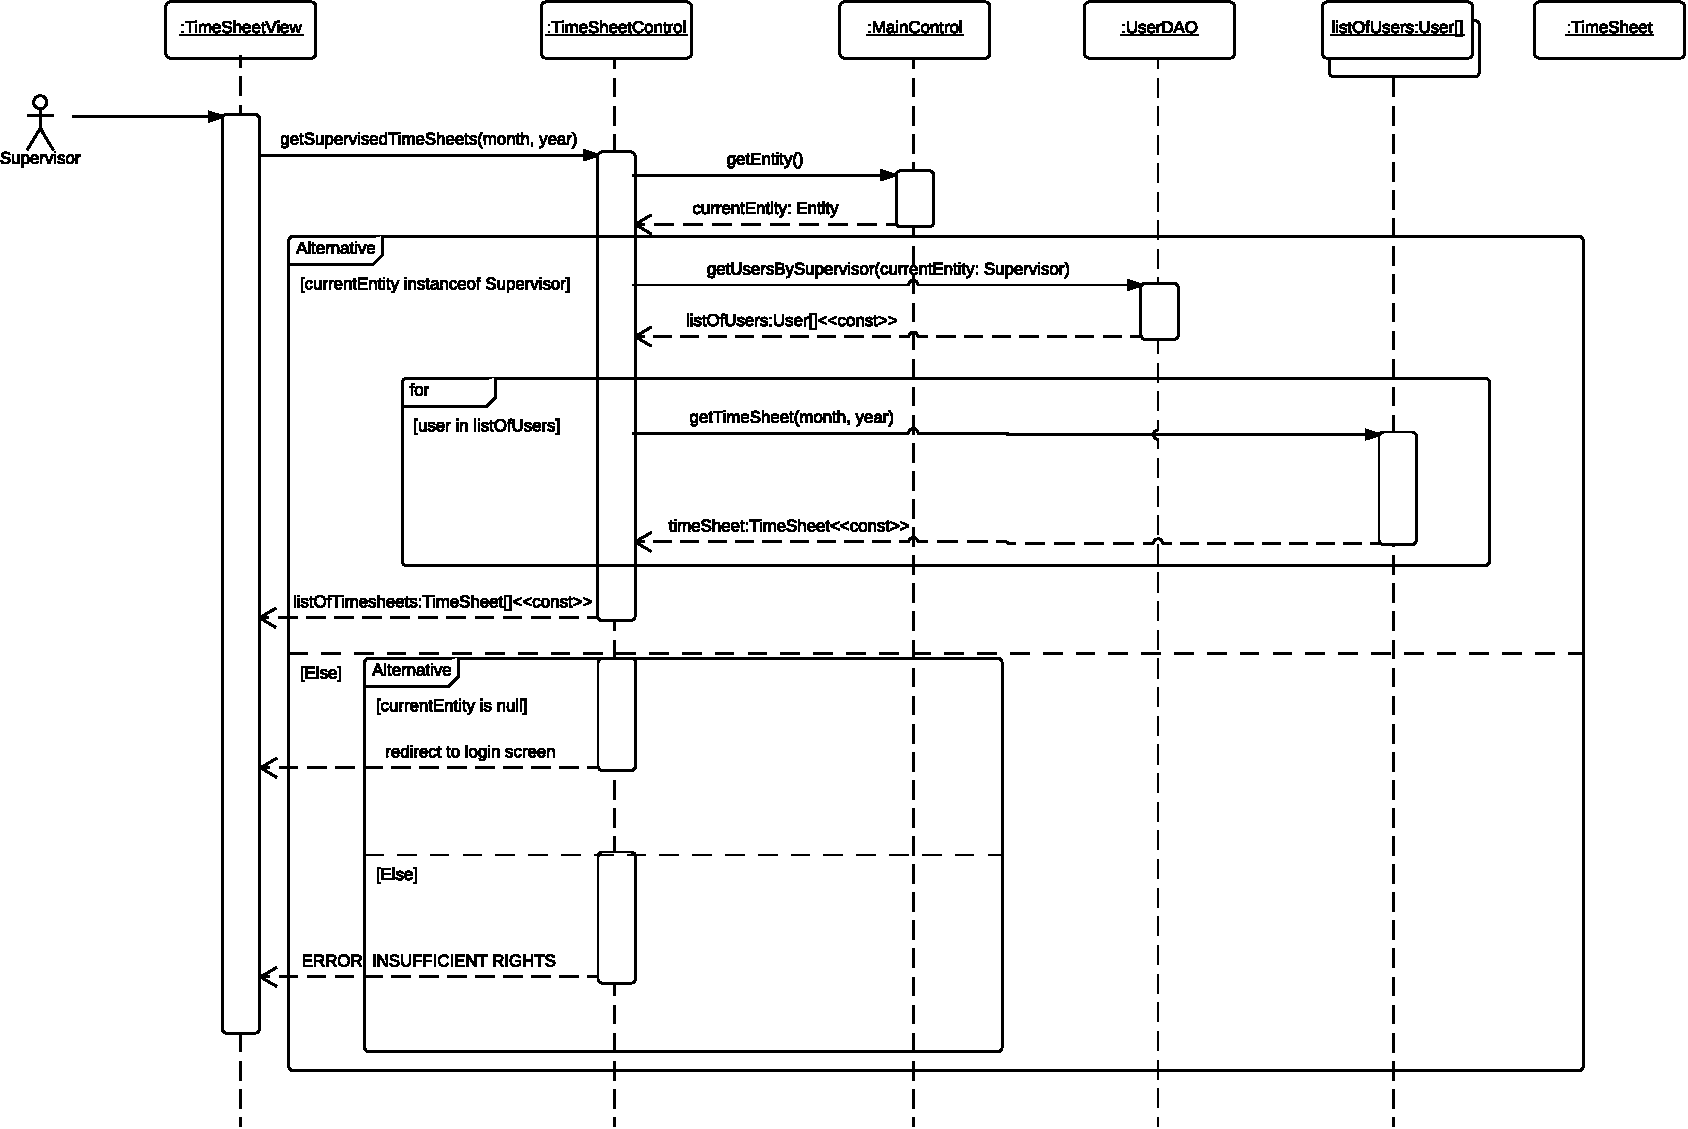
\includegraphics[width=\linewidth]{Diagramms/sequenzes/timesheets_of_all_supervised.pdf}

    \newpage
    \subsection{Aktuellen Stundenzettel einsehen}

        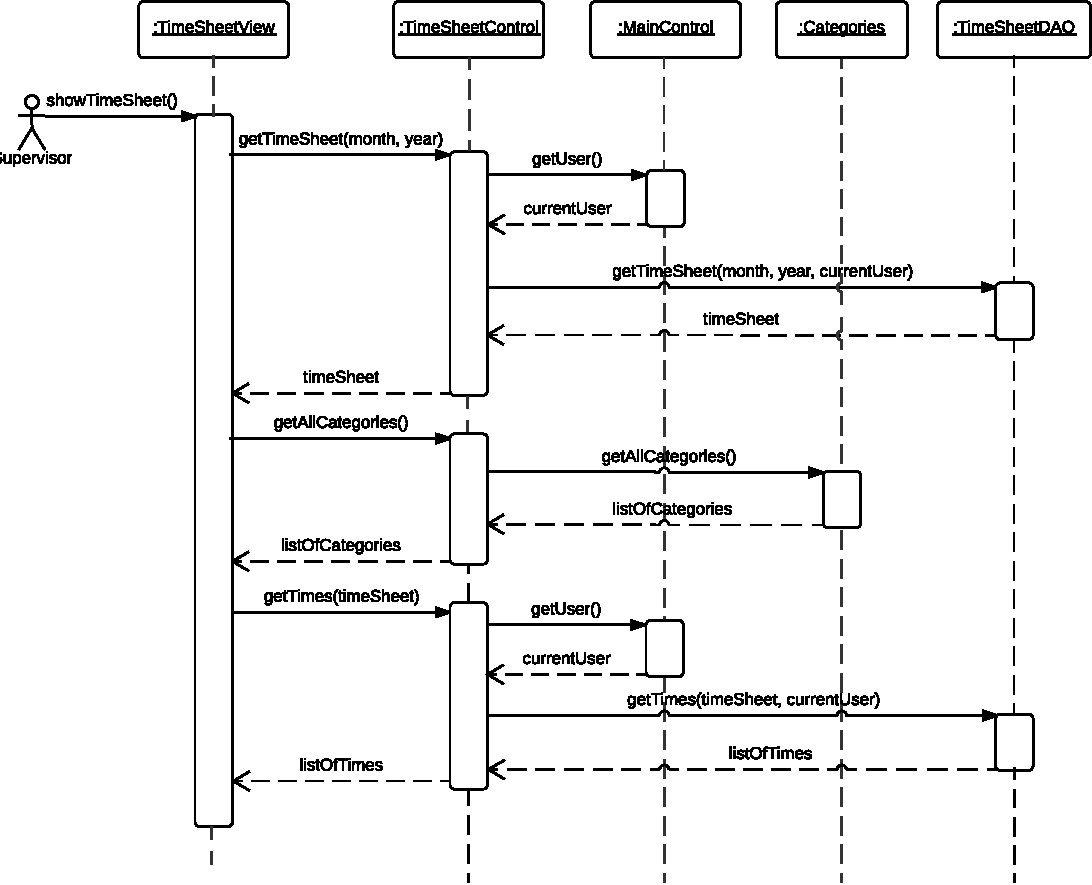
\includegraphics[width=\linewidth]{Diagramms/sequenzes/current_timesheet.pdf}

    \newpage
    \subsection{Stundenzettel abgeben}

        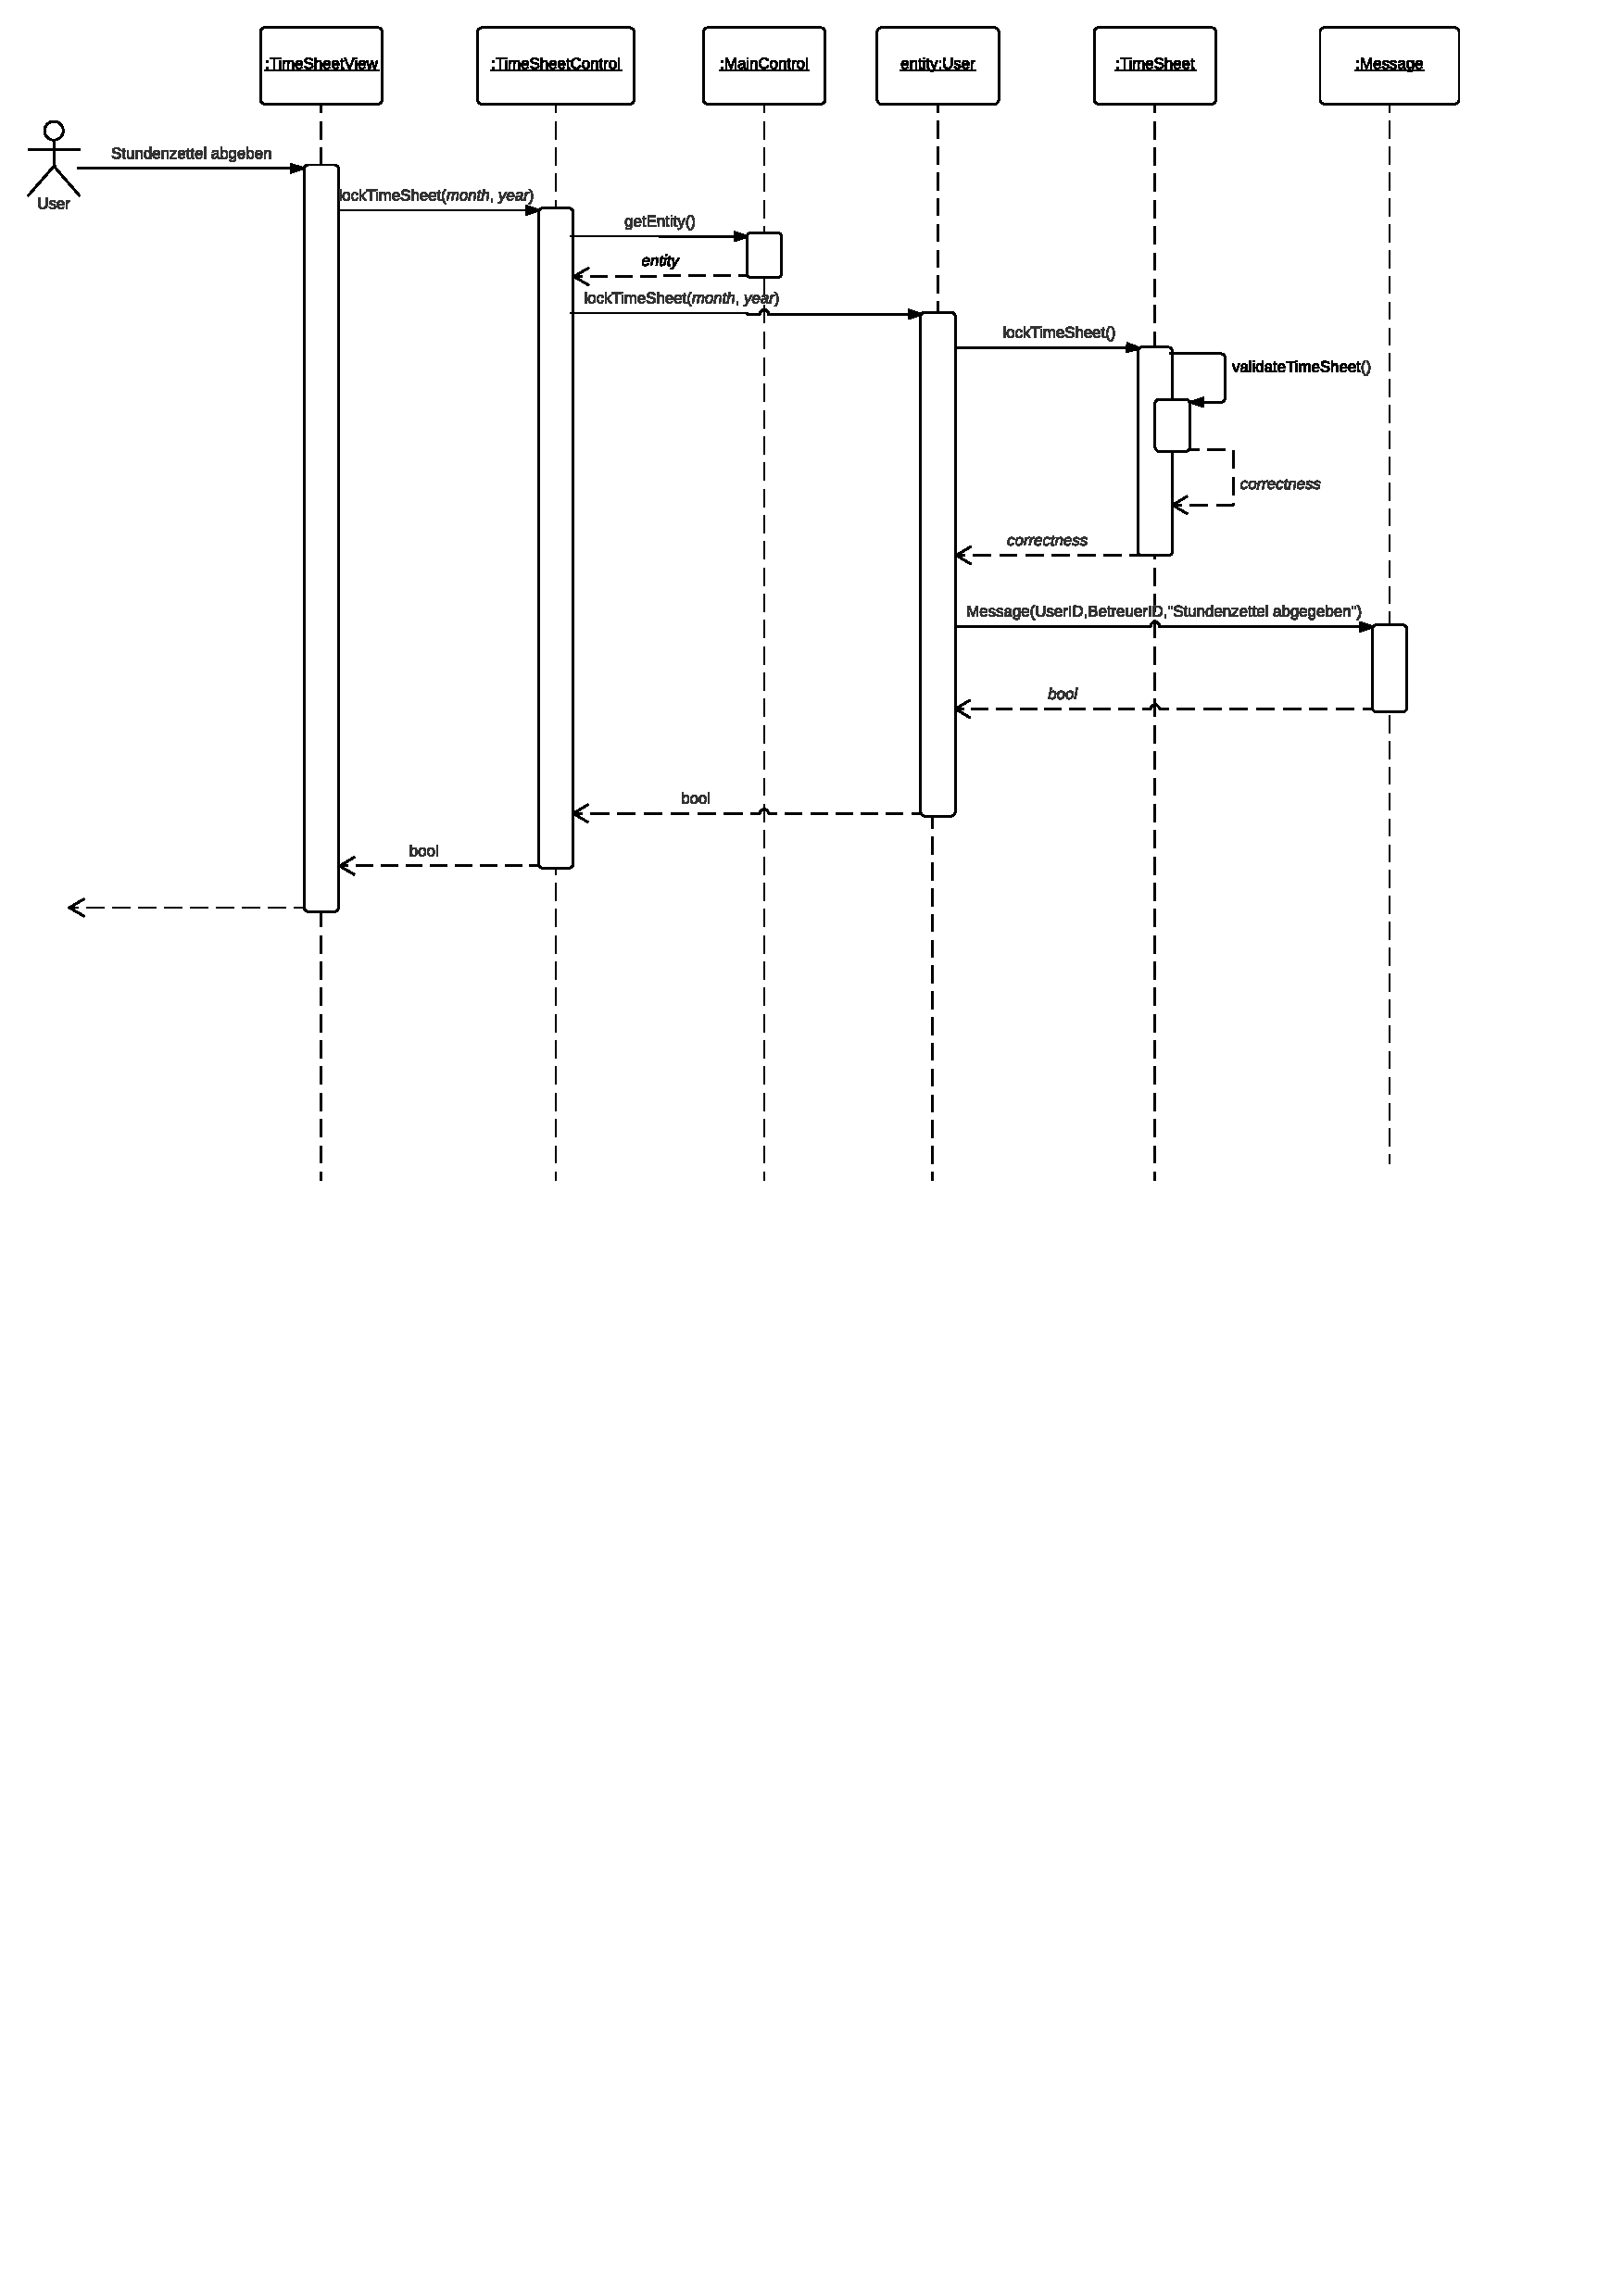
\includegraphics[width=\linewidth]{Diagramms/sequenzes/send_in_timesheet.pdf}

    \newpage
    \subsection{Benutzer anlegen}

        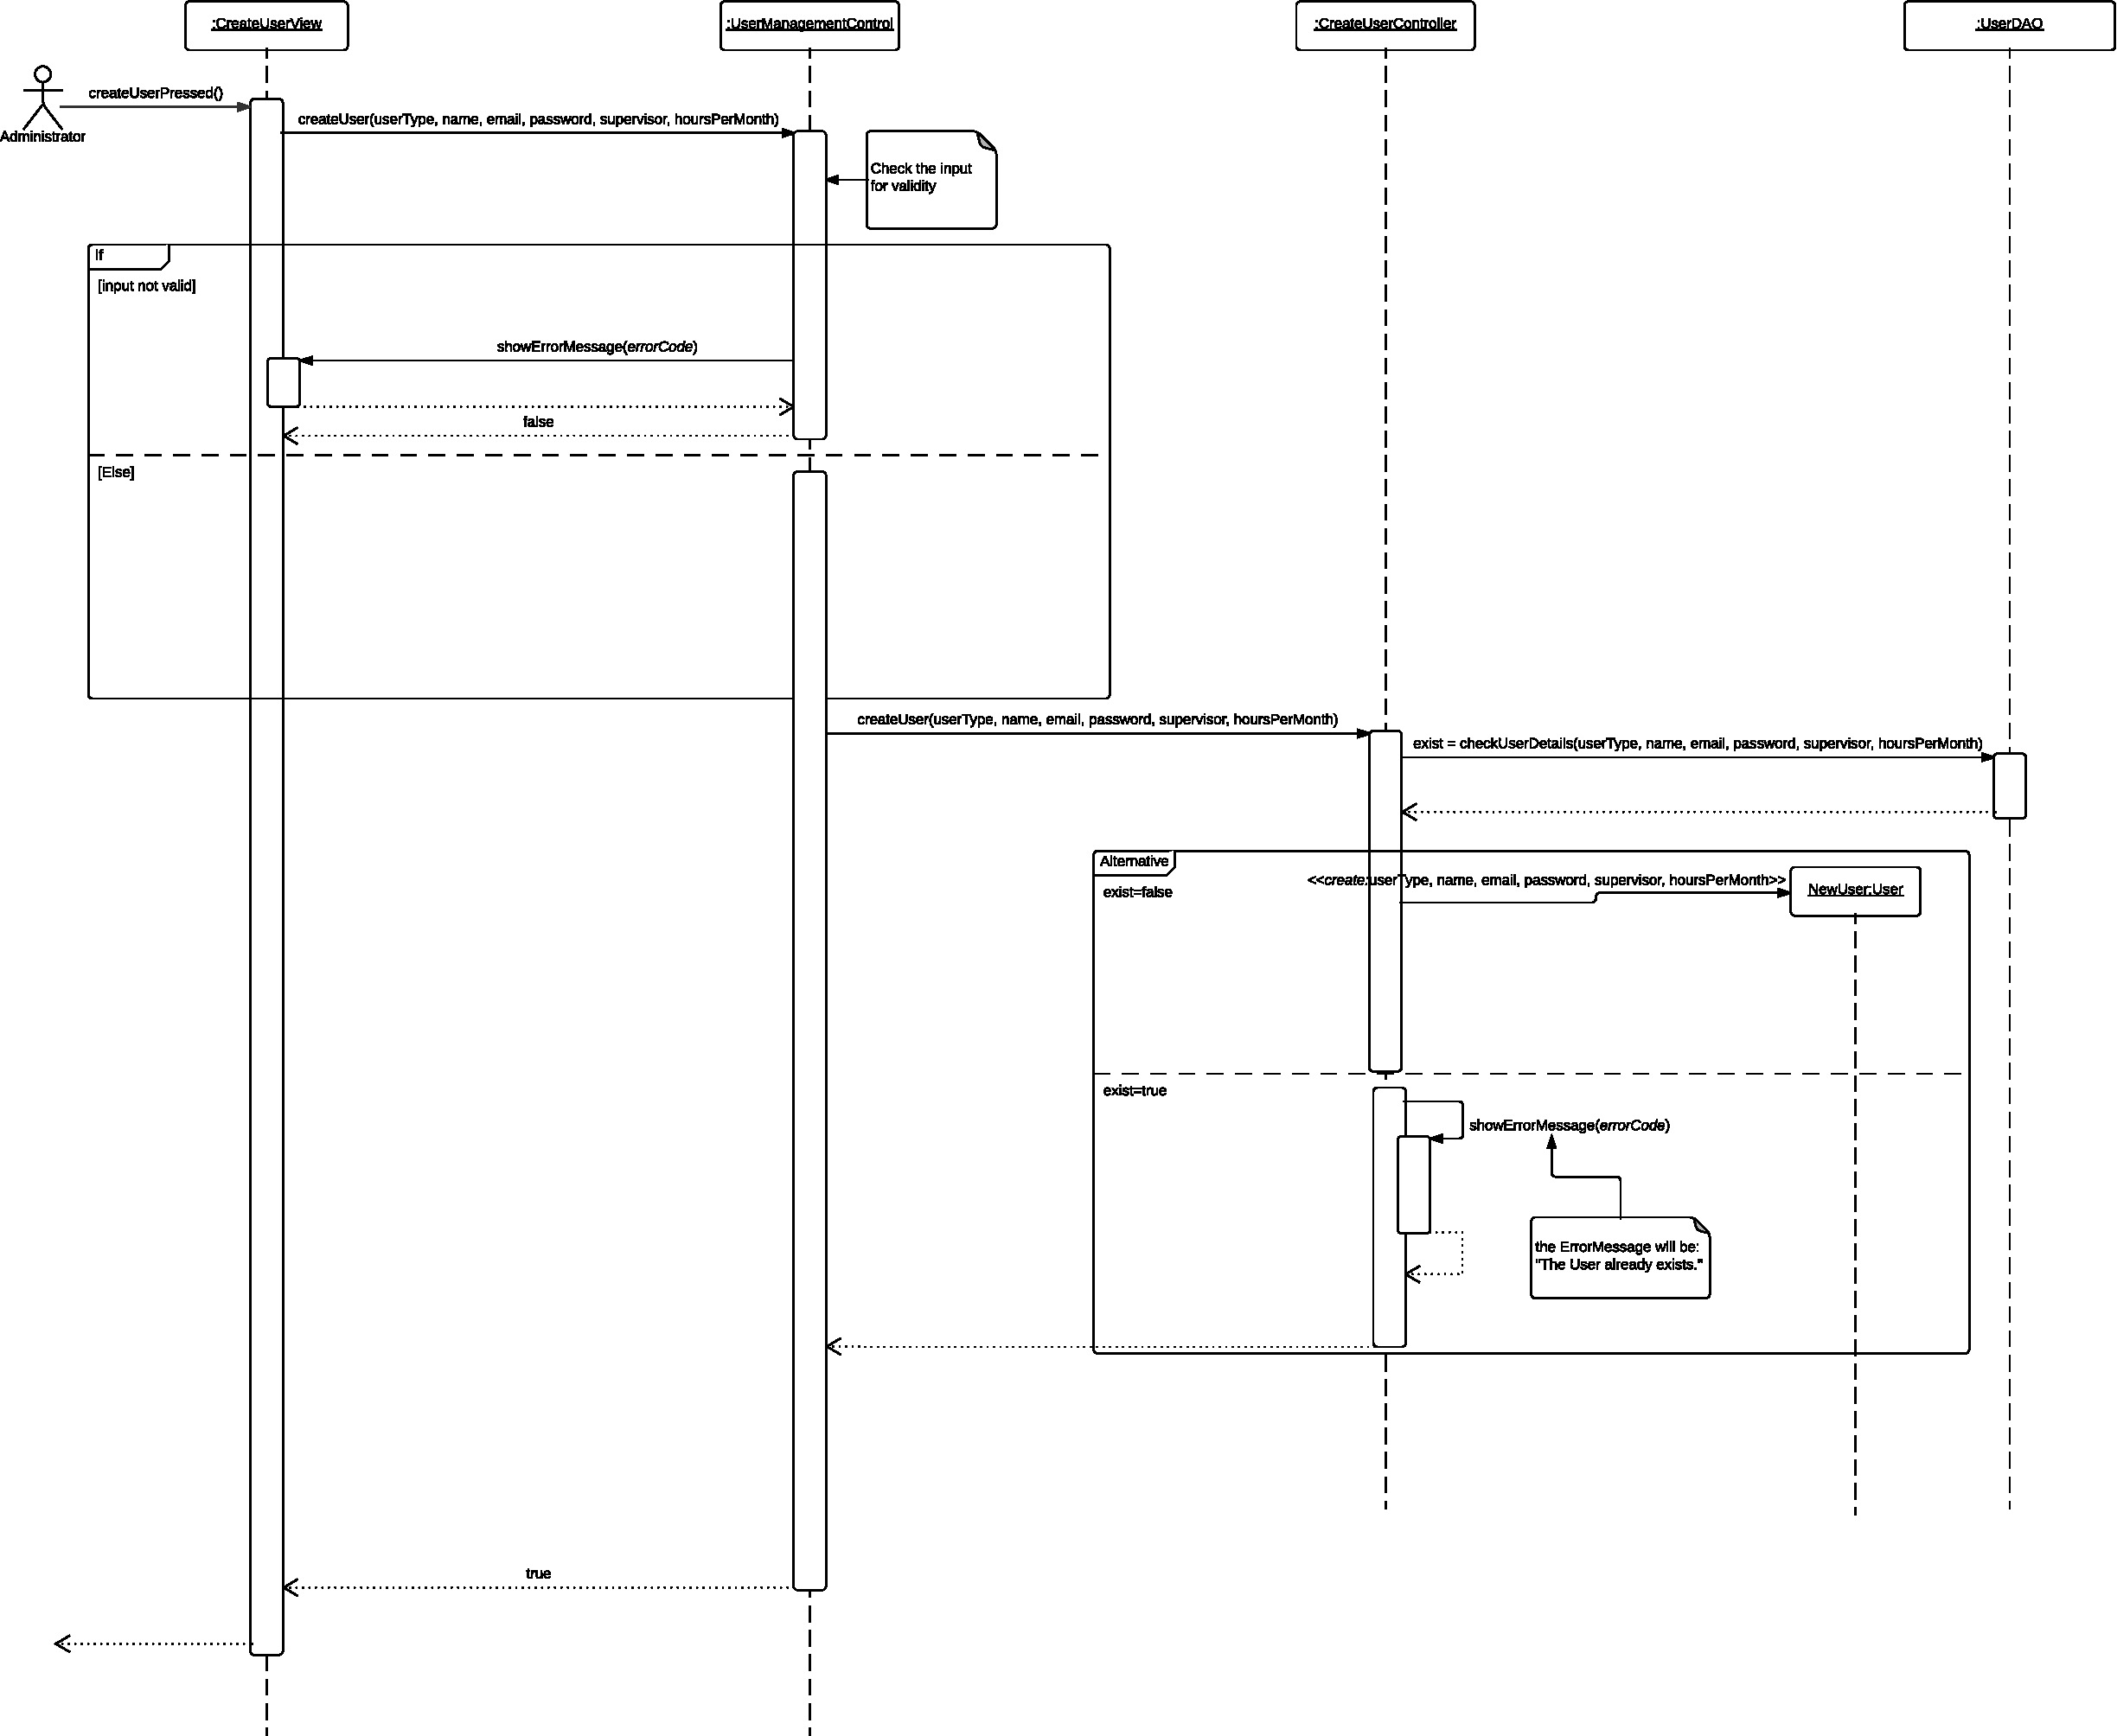
\includegraphics[width=\linewidth]{Diagramms/sequenzes/create_user.pdf}

    \newpage
    \subsection{Nachrichten übermittelung}

        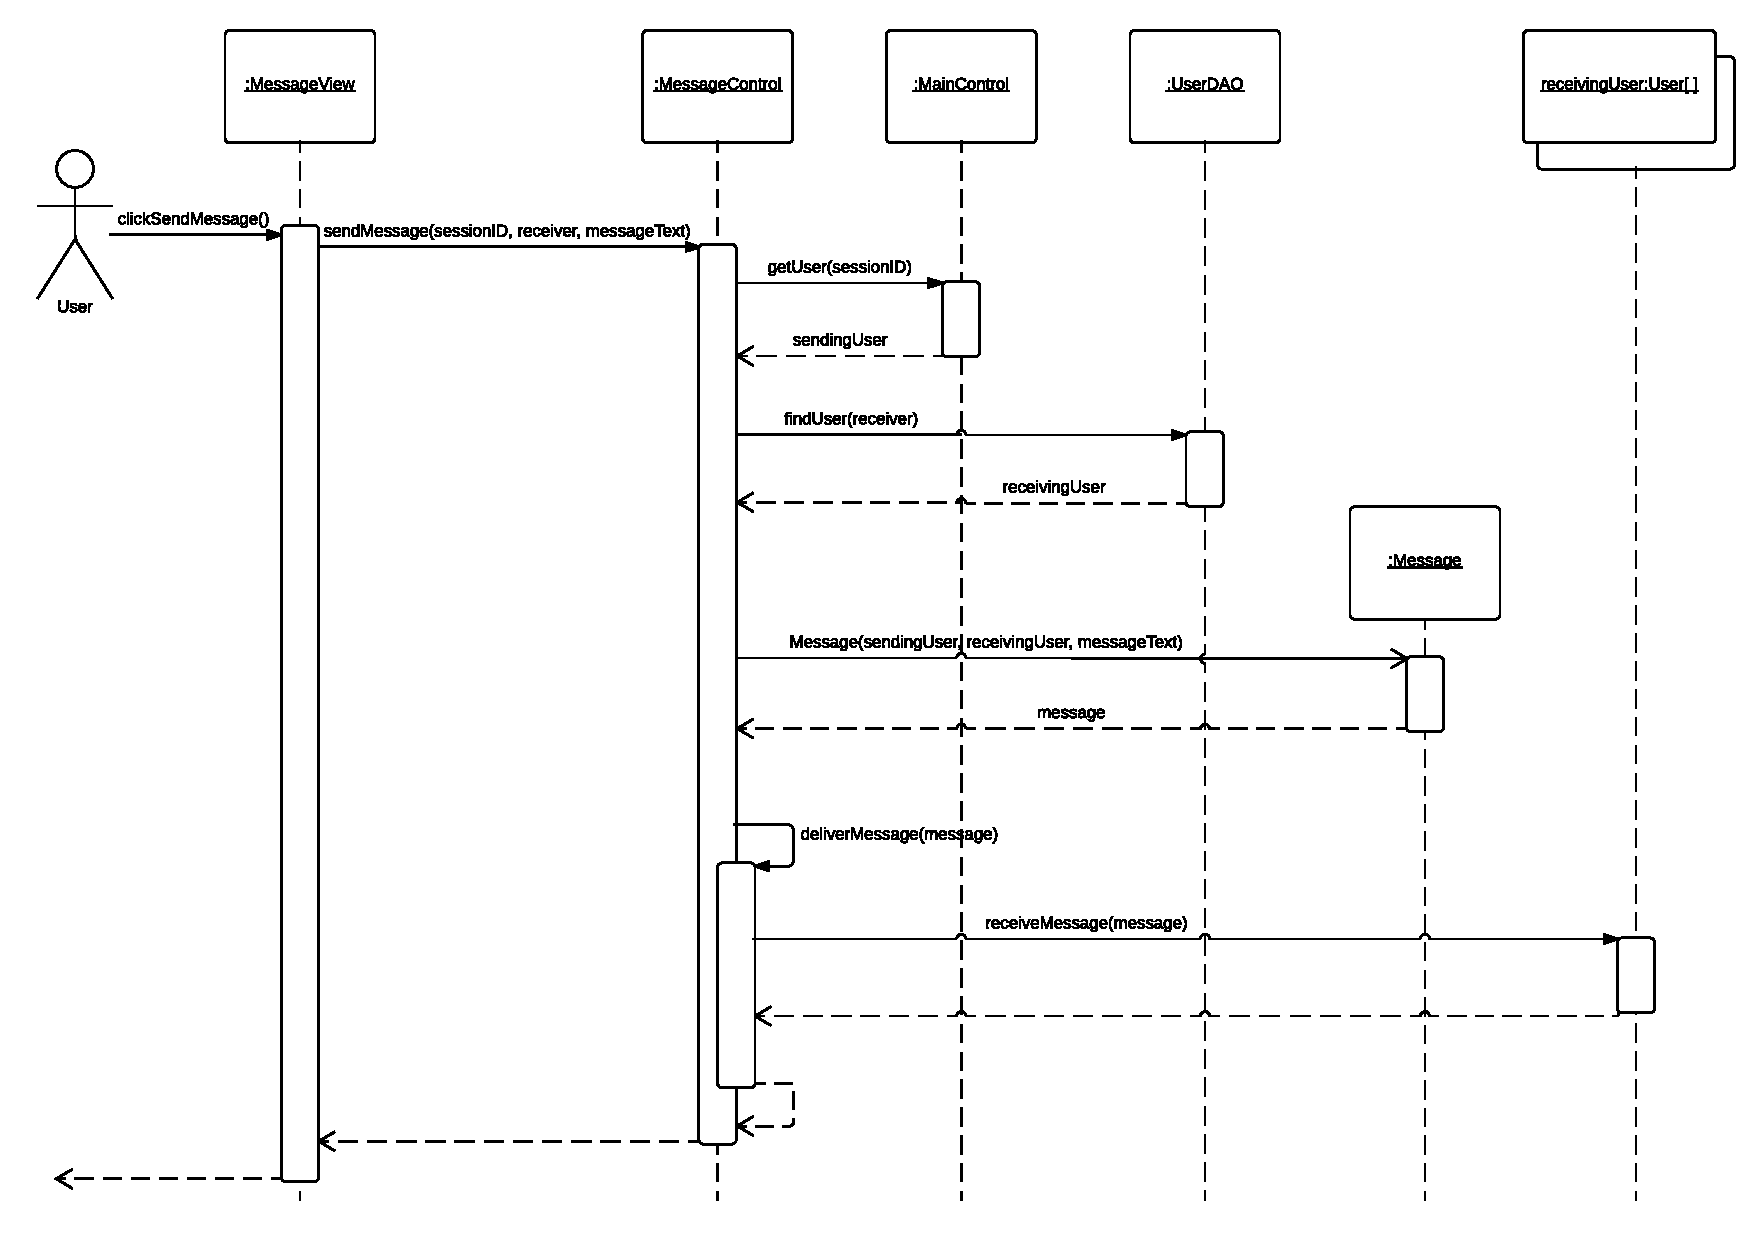
\includegraphics[width=\linewidth]{Diagramms/sequenzes/message_delivery.pdf}

    \newpage
    \subsection{Admin druckt alle Stundenzettel}

        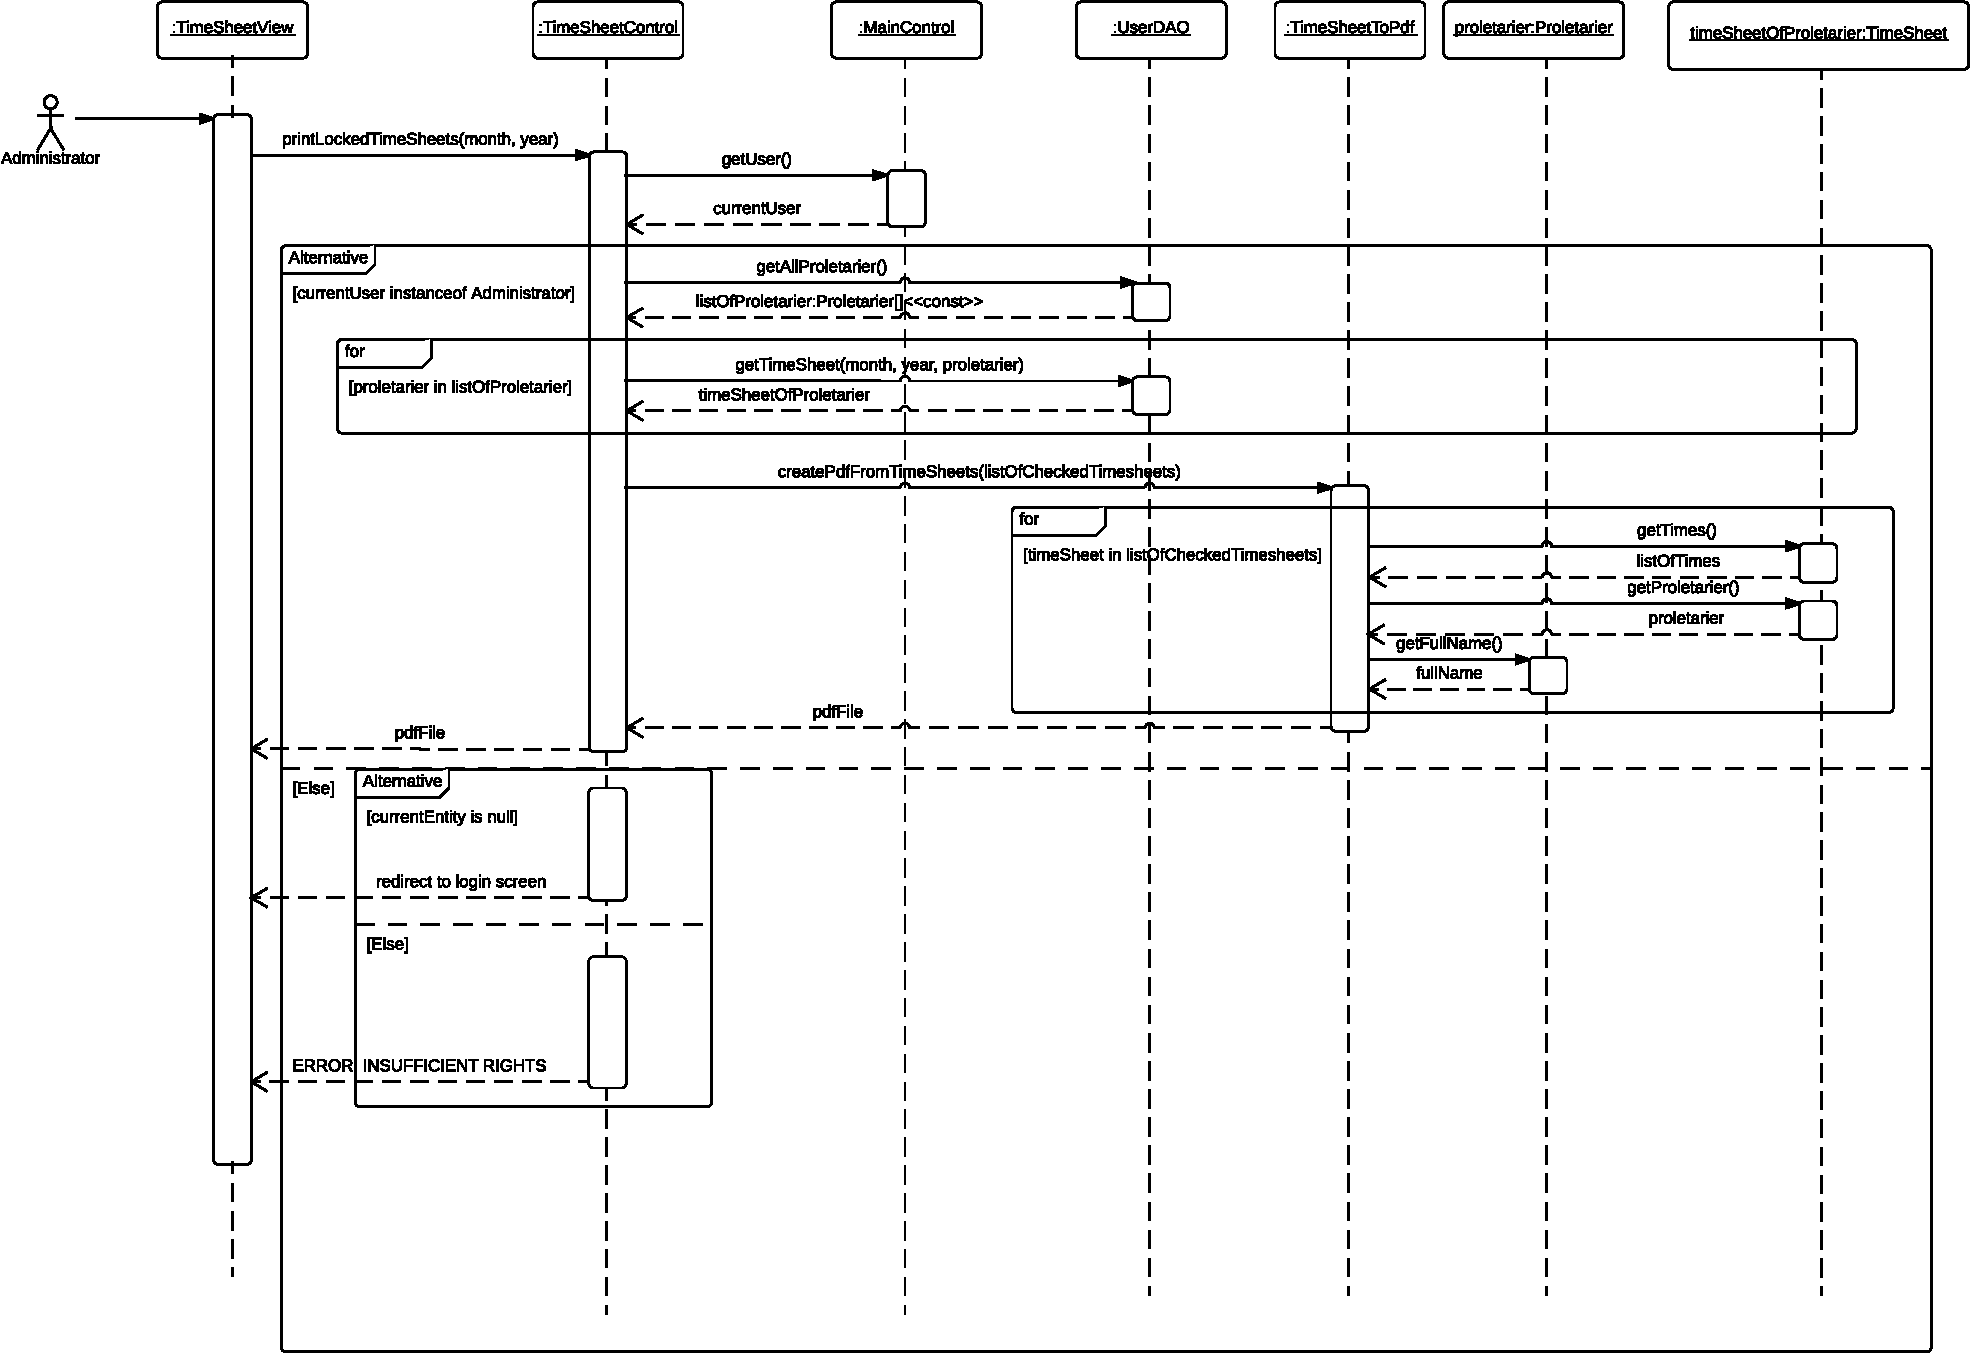
\includegraphics[width=\linewidth]{Diagramms/sequenzes/admin_prints_timesheets.pdf}

    \newpage
    \subsection{Prüfung eines Stundenzettels auf Rechtskonformität}
        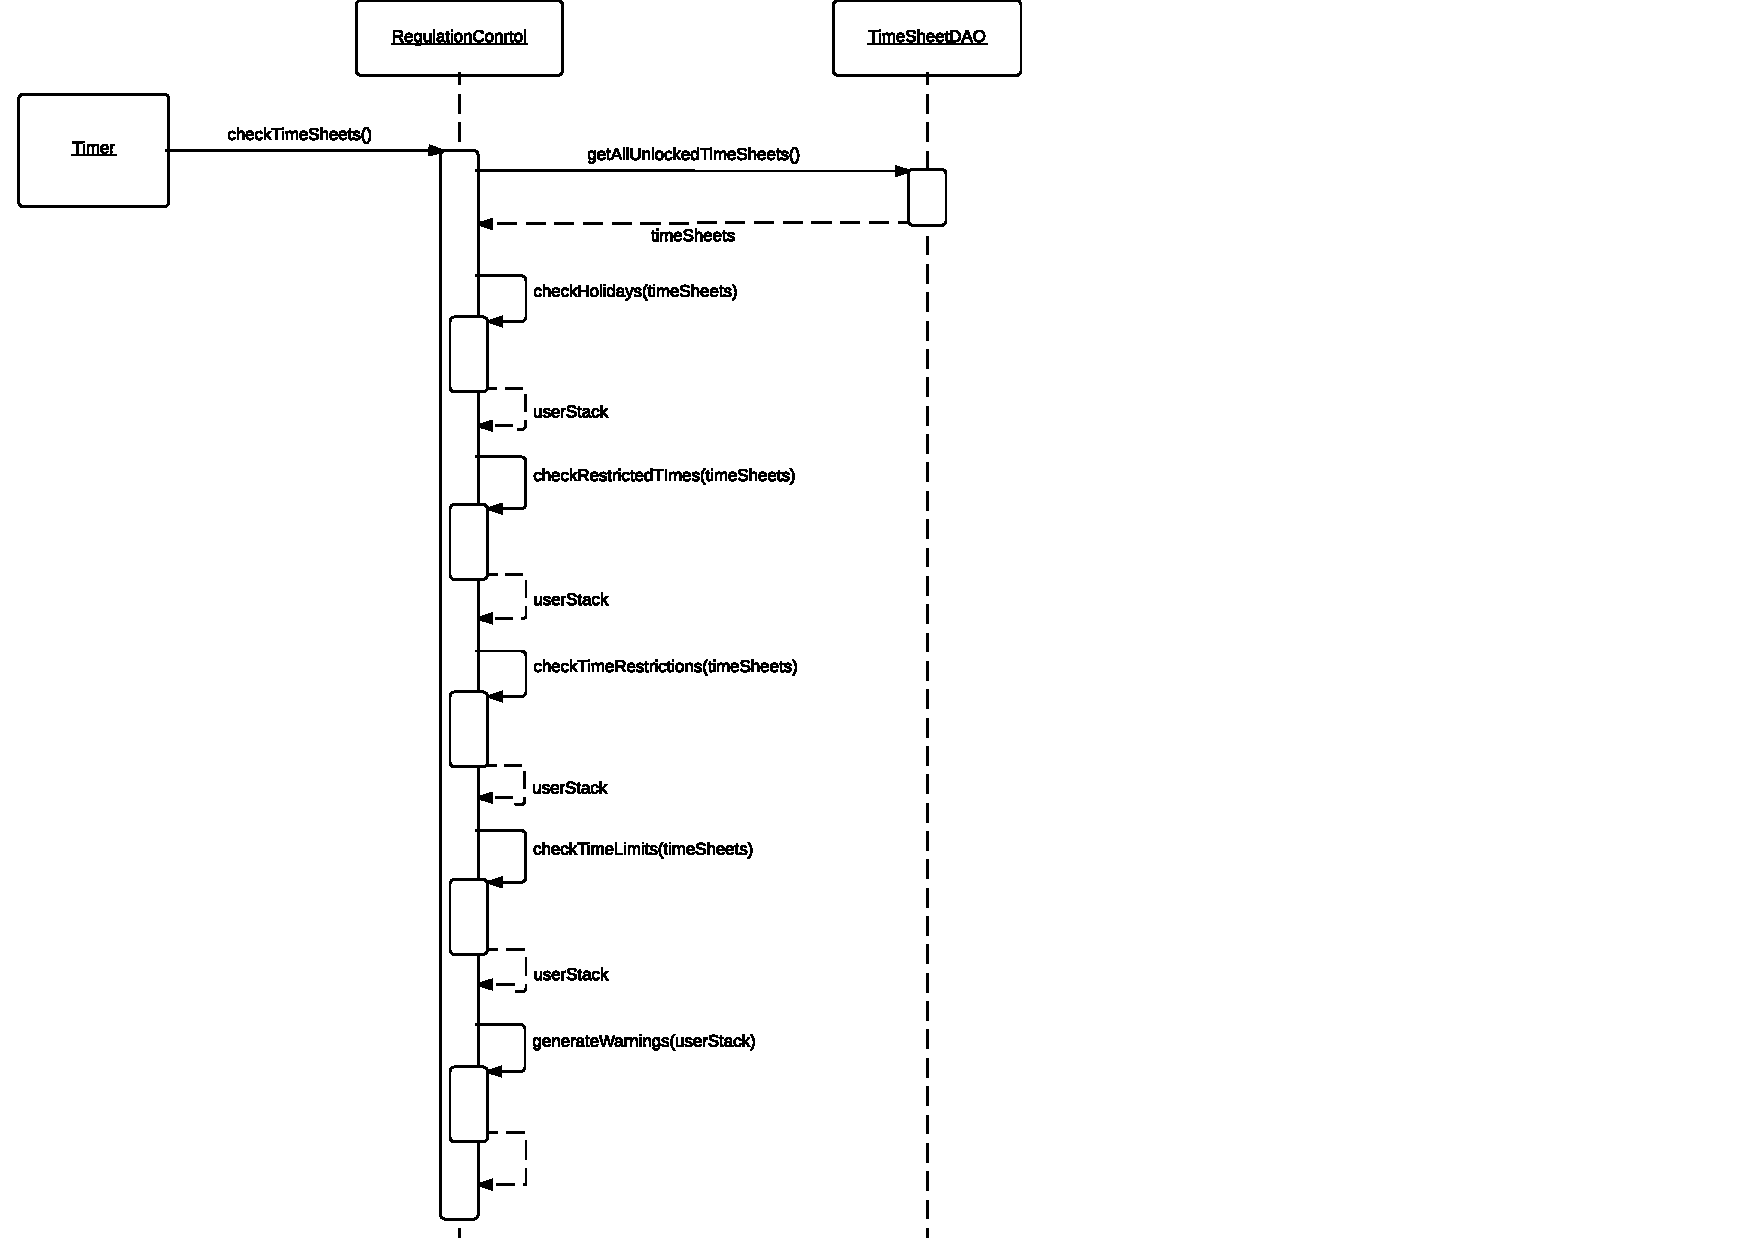
\includegraphics[width=\linewidth]{Diagramms/sequenzes/check_inconsistencies.pdf}


\newpage
